\section{Introducci\'on}

%Poner aca las edos

\section{Implementaci\'on}

%%%%%%%%%%%%%%%%%%%%%
\begin{lstlisting}[language=Matlab, caption=heun.m]
function [x t]=heun(f,x0,t0,tf,n,par)
    h=(tf-t0)/n;
    t=linspace(t0,tf,n);
    x(1,:)=x0;
    for i=1:n-1
        k1(i,:)=f(t(i),x(i,:), par);
        k2(i,:)=f(t(i)+h,x(i,:)+k1(i,:), par);
        x(i+1,:)=x(i,:)+(h/2)*(k1(i,:)+k2(i,:));
    end
\end{lstlisting}

\begin{lstlisting}[language=Matlab, caption=miode.m]
function [x t]=miode(f,x0,t0,tf,dtmax,tol,par)
  n = ceil((tf-t0)/dtmax);
  err = 1;
  
  while (err > tol)
    [x1 t1] = heun(f,x0,t0,tf,n,par); 
    [x2 t2] = heun(f,x0,t0,tf,n*2, par);
    err = max(abs(x1(tf)-x2(tf)));
    n = n + 1;
  end
  
  [x t] = heun(f,x0,t0,tf,n-1,par); 
\end{lstlisting}

\begin{lstlisting}[language=Matlab, caption=ejemplo.m]
f=@(t,y,p) 2*t;

[x t] = miode(f, 1, -2, 2, 1, 10^-1,'a');

plot(t,x)
\end{lstlisting}

\begin{lstlisting}[language=Matlab, caption=edos.m]
clear all;
clc;

I_R=@(t,p) strcmp(p,'a3')*(0.0001).*(20<=t && t<=80)+strcmp(p,'b3')*(-0.00012).*(20<=t && t<=80);

I_B=@(t,p) strcmp(p,'a1')*(0.0001).*(20<=t && t<=80)+strcmp(p,'b1')*(-8.3*10^-5).*(20<=t && t<=80);

I_C=@(t,p) strcmp(p,'a2')*(0.0001).*(20<=t && t<=80)+strcmp(p,'b2')*(-0.00029).*(20<=t && t <= 80);

I_P=@(t,p) strcmp(p,'c1')*(1000).*(20<=t && t<=80);

I_0=@(t,p) strcmp(p,'c2')*(2.5*10^5).*(20<=t && t<= 80);

I_L=@(t,p) strcmp(p,'c3')*(10^4).*(t>=20);

% constantes
k1 = 10^(-2);
k2 = 10;
f0 = 0.05;
d_B = 0.7;
Cs = 5*10^(-3); 
k3 = 5.8 * 10^(-4);
k4 = 1.7 * 10^(-2);
k0 = 0.35;
K = 10;
klp = 3*10^6;
kop = 2*10^5;
r_L = 10^3;
k_P = 86;
S_P = 250;
k6 = 3;
k5 = 0.02;

P0 = S_P / k_P;
Ps = k6 / k5;

D_R = 7*10^(-4);
D_B = f0 * d_B; 
k_B = 0.189;
D_C = 2.1*10^(-3);
D_A = 0.7;
R = 0.0007734;
B = 0.0007282;
C = 0.0009127;

pi_C = @(t,y,p) (y(3) + f0 * Cs)/(y(3) + Cs);
P_ = @(t,p) I_P(t,p) / k_P;
pi_p = @(t,p) (P_(t,p) + P0)/(P_(t,p) + Ps);
pi_L = @(t,y,p) (k3/k4)*((klp * pi_p(t,p) * y(2))/(1 + (k3*K/k4) + (k1/(k2*k0))*(((kop/pi_p(t,p))*y(1)) + I_0(t,p) ))) * (1 + (I_L(t,p)/r_L));


f=@(t,y,p)[
    D_R*pi_C(t,y,p)-(D_B/pi_C(t,y,p))*y(1)+I_R(t,p),D_B/pi_C(t,y,p)*y(1)-k_B*y(2)+I_B(t,p),D_C*pi_L(t,y,p)-D_A*pi_C(t,y,p)*y(3)+I_C(t,p)
   ];


[x t] = miode(f, [R B C], 0, 140, 1, 10^-6,'a1');
plot(t, x)
[x t] = miode(f, [R B C], 0, 140, 1, 10^-6,'a2');
plot(t,x)
[x t] = miode(f, [R B C], 0, 140, 1, 10^-6,'a3');
plot(t,x)
[x t] = miode(f, [R B C], 0, 140, 1, 10^-6,'b1');
plot(t,x)
[x t] = miode(f, [R B C], 0, 140, 1, 10^-6,'b2');
plot(t,x)
[x t] = miode(f, [R B C], 0, 140, 1, 10^-6,'b3');
plot(t,x)
[x t] = miode(f, [R B C], 0, 140, 1, 10^-6,'c1');
plot(t,x)
[x t] = miode(f, [R B C], 0, 140, 1, 10^-6,'c2');
plot(t,x)
[x t] = miode(f, [R B C], 0, 140, 1, 10^-6,'c3');
plot(t,x)

\end{lstlisting}

\section{Resultados}

\begin{figure}[h!]
\centering
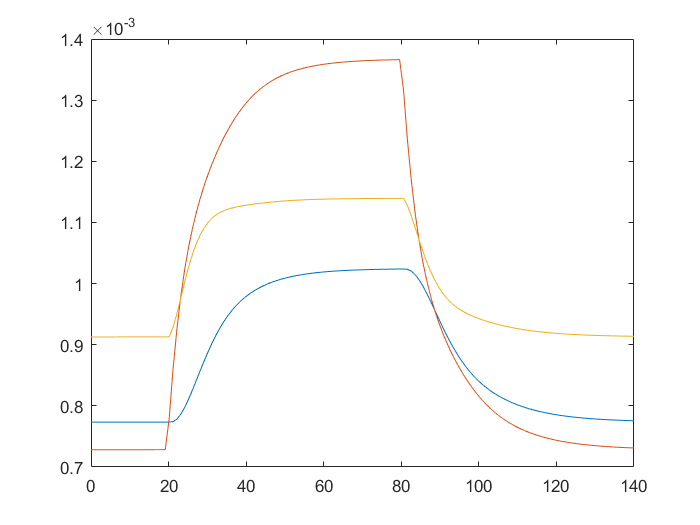
\includegraphics[scale=0.3]{../a1.png}\hspace{0.01cm}
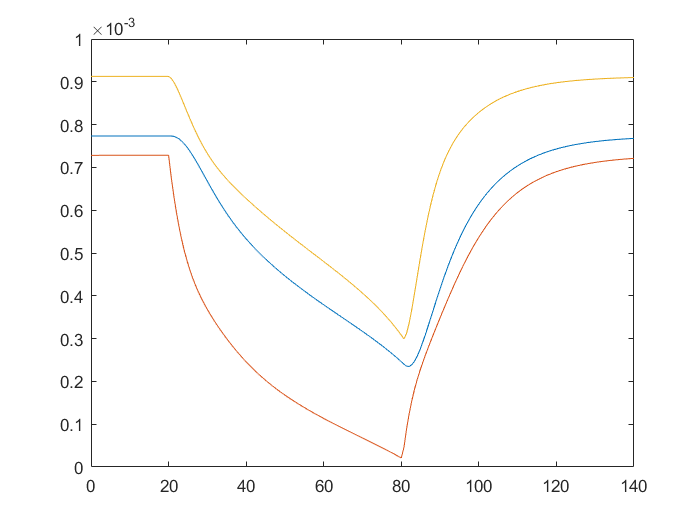
\includegraphics[scale=0.3]{../b1.png}\hspace{0.01cm}
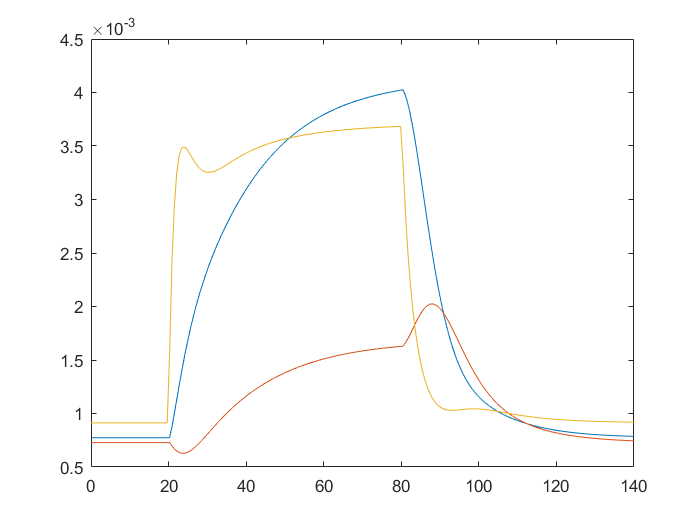
\includegraphics[scale=0.3]{../c1.png}\\
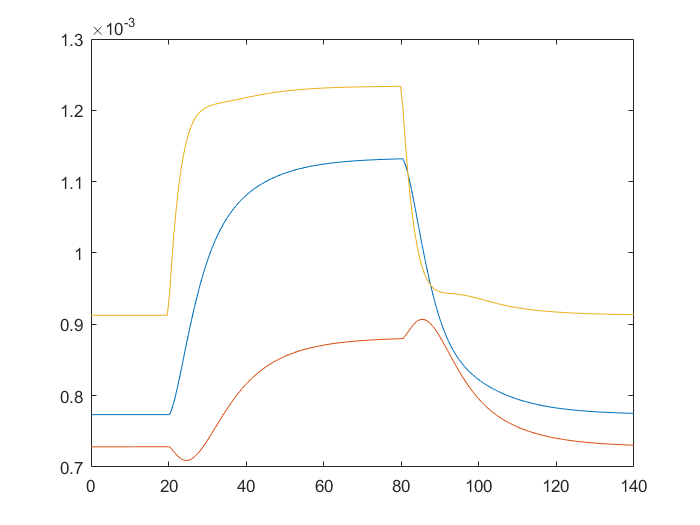
\includegraphics[scale=0.3]{../a2.png}\hspace{0.01cm}
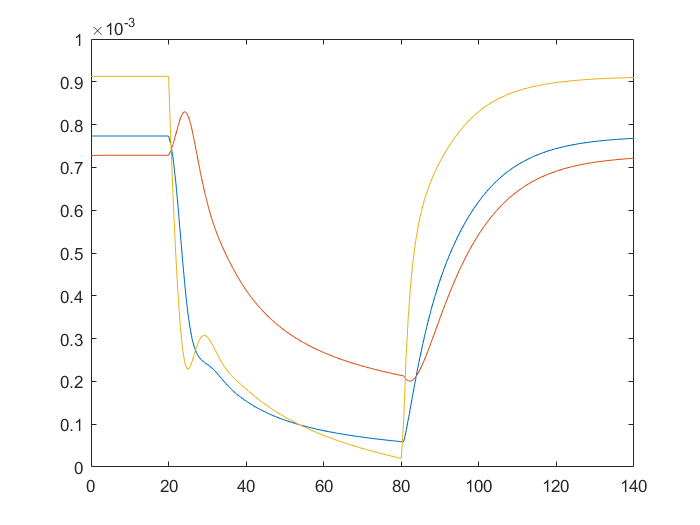
\includegraphics[scale=0.3]{../b2.png}\hspace{0.01cm}
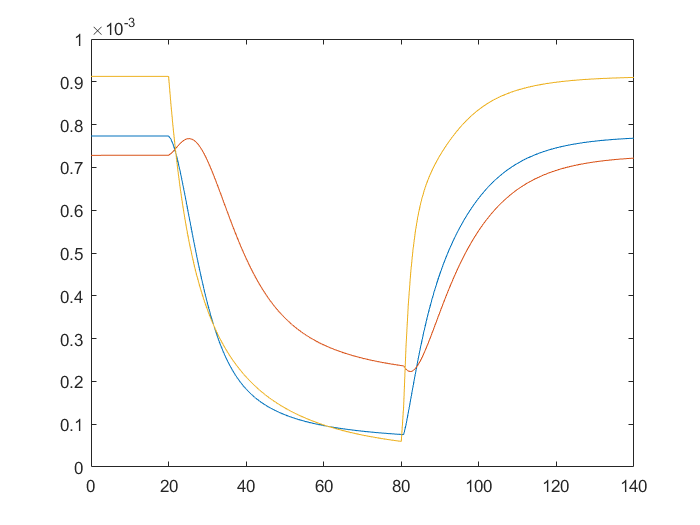
\includegraphics[scale=0.3]{../c2.png}\\
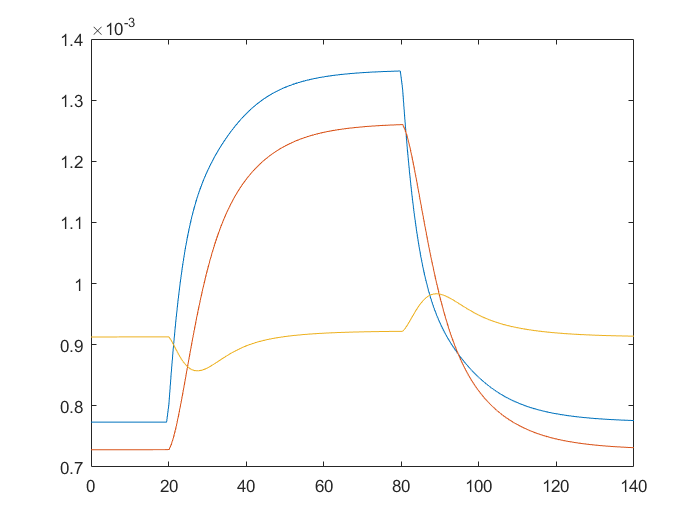
\includegraphics[scale=0.3]{../a3.png}\hspace{0.01cm}
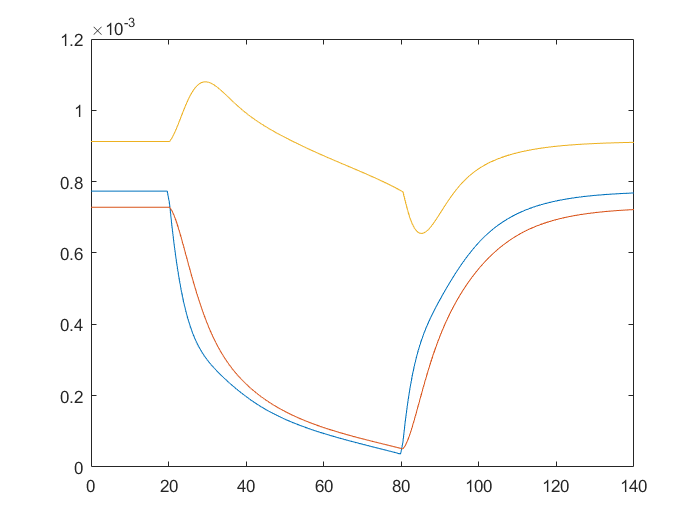
\includegraphics[scale=0.3]{../b3.png}\hspace{0.01cm}
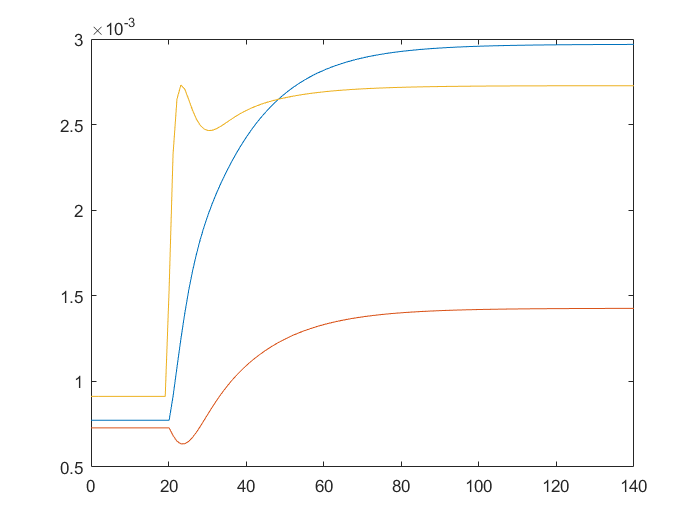
\includegraphics[scale=0.3]{../c3.png}
\caption{Resultados de las EDOs.}
\label{circnpnmaxout}
\end{figure}

